% cd /storage/emulated/0/Documents/documents/latex/1920/Grade-10/1st/power-theorems && pdflatex ps-power-theorems.tex && termux-open ps-power-theorems.pdf

% cd /storage/emulated/0/Documents/documents/latex/1920/Grade-10/1st/power-theorems && clean-tex ps-power-theorems-input1.tex


% cd /storage/emulated/0/Documents/documents/latex/1920/Grade-10/1st/power-theorems && convert -density 600 ps-power-theorems.pdf -crop 2200x1700 -quality 100 -verbose ps-power-theorems%02d.png

%2480.5x3508 portrait 2x2 2550x3300
%3508x2480.5 landscape 2x2 3300x2550 
%1653.7x2338.7 portrait 3x3 1700x2200
%landscape 3x3 2200x1700

% cd /storage/emulated/0/Documents/documents/latex/1819/grade10/visual/4th/power-theorems && while inotifywait -e close_write ps-power-theorems*.tex; do touch /storage/emulated/0/Android/data/com.termux/files/launch-termux.txt && printf '1' > /storage/emulated/0/Android/data/com.termux/files/launch-termux.txt && pdflatex ps-power-theorems.tex && termux-open ps-power-theorems.pdf; done

% cd /host-rootfs/storage/emulated/0/Documents/documents/latex/1819/grade10/visual/4th/power-theorems && while inotifywait -e close_write ps-power-theorems*.tex; do pdflatex ps-power-theorems.tex  && printf "/storage/emulated/0/Documents/documents/latex/1819/grade10/visual/4th/power-theorems/ps-power-theorems.pdf" > /host-rootfs/storage/emulated/0/GNURoot/home/Scripts/file-to-launch.txt; done


\documentclass[10pt]{article}
\usepackage[letterpaper, landscape, right=0.25in, left=0.25in, top=0.25in, bottom=0.25in]{geometry}
\usepackage{xcolor}
\usepackage{anyfontsize}
\usepackage{enumitem}
\usepackage{multicol}
\usepackage{amsmath}
%\usepackage{amsfonts,dsfont}% for \mathds 
\usepackage{tabularx} 
\usepackage{gensymb}
\usepackage{multirow}
\usepackage{graphicx, tipa}
\usepackage{tikz}
\usetikzlibrary{angles,quotes}
\usepackage{pgfplots} 
\usetikzlibrary{calc}
\pgfplotsset{compat=newest}
\usetikzlibrary{arrows.meta}
\usetikzlibrary{intersections}
\usetikzlibrary{decorations.pathreplacing}
\usepackage{flafter}
\usepackage{amsmath,amssymb,cancel,units}
\usepackage{microtype} % nicer output 
\usepackage{hfoldsty} % nicer output 
\usepackage{fixltx2e} 
\usepackage{mathptmx}
%\usepackage{booktabs}
\usepackage{numprint}
\usepackage[utf8]{inputenc} 
\usepackage[T1]{fontenc}
%\usepackage{siunitx} 
%\sisetup{detect-all}


\def\radA{3.6cm}

\def\radB{3.6cm}

%\def\thirdrad{8cm}

\pagenumbering{gobble}
%\linespread{0.9}
\newcommand{\vspce}{\vspace{0.75ex}}
\newcommand{\hspce}{\hspace{0.5em}}
\newcommand{\blank}{\underline{\hspace{2em}}}%{\rule{1em}{0.15ex}}
\newcommand{\arc}[1]{{% 
\setbox9=\hbox{#1}% 
\ooalign{\resizebox{\wd9}{\height}{\texttoptiebar{\phantom{A}}}\cr#1}}}

\newcolumntype{C}{ >{\centering\arraybackslash} X}




\begin{document}
\boldmath
{\fontsize{36}{40}\fontfamily{pnc}\selectfont {

\def\curdir{/storage/emulated/0/Documents/documents/latex/1920/Grade-10/2nd/power-theorems}
\def\radA{1cm}

\textbf{Practice Exercises}

\vspce

Find the value of $x$. 
\begin{center}
%\vspace*{-2ex}
\scalebox{0.8}{
\noindent\begin{minipage}{\textwidth}
{\begin{tabularx}{\textwidth}{XX}
1. 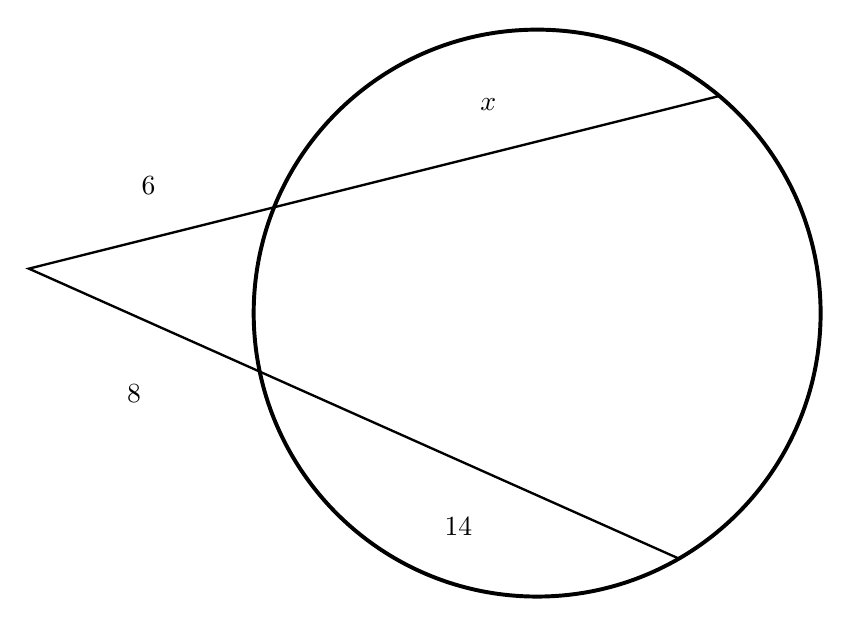
\begin{tikzpicture}[dot/.style={circle, fill=black, inner sep=0pt, outer sep=0pt, minimum size=3pt}, baseline = (current bounding box.west)]

\coordinate (circ) at (0,0); 

\draw[name path=circum, line width=0.5mm] (circ) circle (\radA);

\coordinate (a) at ($(circ) + (50:\radA)$); 

\coordinate (b) at ($(circ) + (175:1.8*\radA)$); 

\coordinate (c) at ($(circ) + (-60:\radA)$); 

\draw[name path=line1, line width=0.3mm] (a) -- (b) -- (c) ;

\fill[black, name intersections={of=line1 and circum, name=int}];

\node(6.label) at ($(int-2)+(170:0.45*\radA)$) {$  6$};

\node(8.label) at ($(int-3)+(190:0.45*\radA)$) {$  8$};

\node(x-label) at ($(a)!0.5!(int-2) +(100:0.17*\radA)$) {$  x$}; 

\node(14-label) at ($(c)!0.5!(int-3) +(-100:0.22*\radA)$) {$  14$}; 

\end{tikzpicture} 

 & 5. 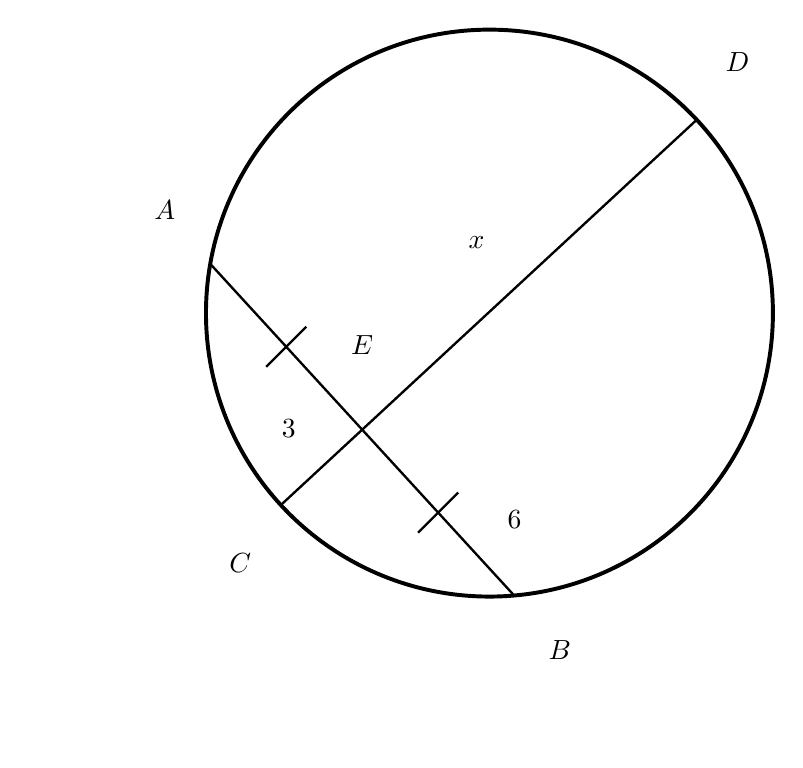
\begin{tikzpicture}[dot/.style={circle, fill=black, inner sep=0pt, outer sep=0pt, minimum size=3pt}, baseline = (current bounding box.west)]

\coordinate (circ) at (0,0); 

\draw[name path=circum, line width=0.5mm] (circ) circle (\radA);

\coordinate (a) at ($(circ) + (170:\radA)$); 

\coordinate (b) at ($(circ) + (275:\radA)$); 

\coordinate (d) at ($(circ) + (43:\radA)$); 

\coordinate (e) at ($(a)! 0.5!(b)$); 

\draw[name path=line1, line width=0.3mm] (a) -- (b);

\path[name path=line.guess, line width=0.3mm] (e) -- ($(e)!1!180:(d)$); 

\fill[black, name intersections={of=circum and line.guess, name=int}];

\coordinate (tick1) at ($(a)! 0.5!(e)$);

\coordinate (tick2) at ($(b)! 0.5!(e)$);  

\tikzset{onetick/.pic={\draw[line width=0.3mm] ($(0,0)+(0,0.1*\radA)$) -- ($(0,0)-(0,0.1*\radA)$) ; }}

\pic[rotate=135] at (tick1) [pic type = onetick];  

\pic[rotate=135] at (tick2) [pic type = onetick];  

\node(6.label) at ($(tick2)+(-5:0.27*\radA)$) {$ 6$};

\node(3.label) at ($(e)! 0.5!(int-1)+(130:0.18*\radA)$) {$ 3$};

\node(x-label) at ($(d)!0.5!(int-1) +(100:0.25*\radA)$) {$ x$}; 

\node(e-label) at ($(e)+(90:0.3*\radA)$) {$ E$}; 

\node(d-label) at ($(d)+(55:0.25*\radA)$) {$ D$}; 

\node(a-label) at ($(a)+(130:0.25*\radA)$) {$ A$};

\node(b-label) at ($(b)-(130:0.25*\radA)$) {$ B$}; 

\node(c-label) at ($(int-1)-(55:0.25*\radA)$) {$ C$}; 

\draw[line width=0.3mm] (int-1) -- (d);

\end{tikzpicture} 
 \\
2. 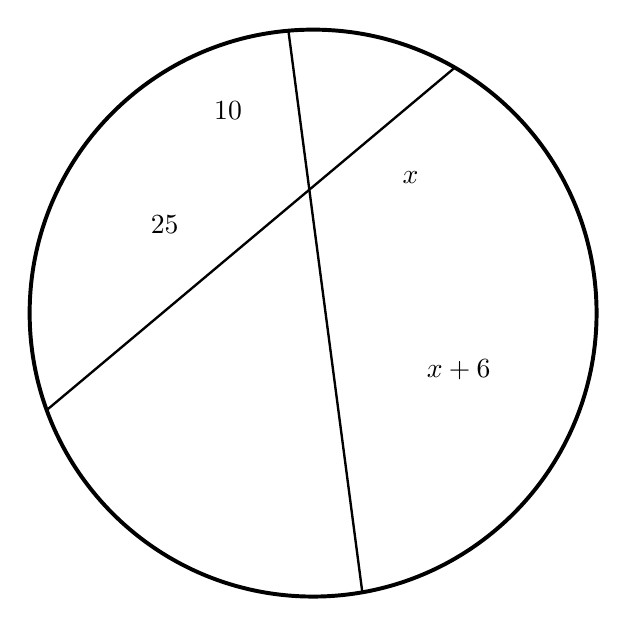
\begin{tikzpicture}[dot/.style={circle, fill=black, inner sep=0pt, outer sep=0pt, minimum size=3pt}, baseline = (current bounding box.west)]

\coordinate (circ) at (0,0); 

\draw[name path=circum, line width=0.5mm] (circ) circle (\radA);

\coordinate (a) at ($(circ) + (95:\radA)$); 

\coordinate (b) at ($(circ) + (-80:\radA)$); 

\coordinate (c) at ($(circ) + (60:\radA)$); 

\coordinate (d) at ($(circ) + (200:\radA)$); 

\draw[name path=line1, line width=0.3mm] (a) -- (b);

\draw[name path=line2, line width=0.3mm] (c) -- (d);

\fill[black, name intersections={of=line1 and line2, name=int}];

\node(10.label) at ($(a)!0.5!(int-1) + (180:0.25*\radA)$) {$  10$};

\node(x.label) at ($(c)!0.5!(int-1) +(-60:0.2*\radA)$) {$  x$};

\node(25-label) at ($(d)!0.5!(int-1) +(100:0.27*\radA)$) {$  25$}; 

\node(x6-label) at ($(b)!0.5!(int-1) +(10:0.44*\radA)$) {$  x+6$}; 

\end{tikzpicture} 
 & 6. 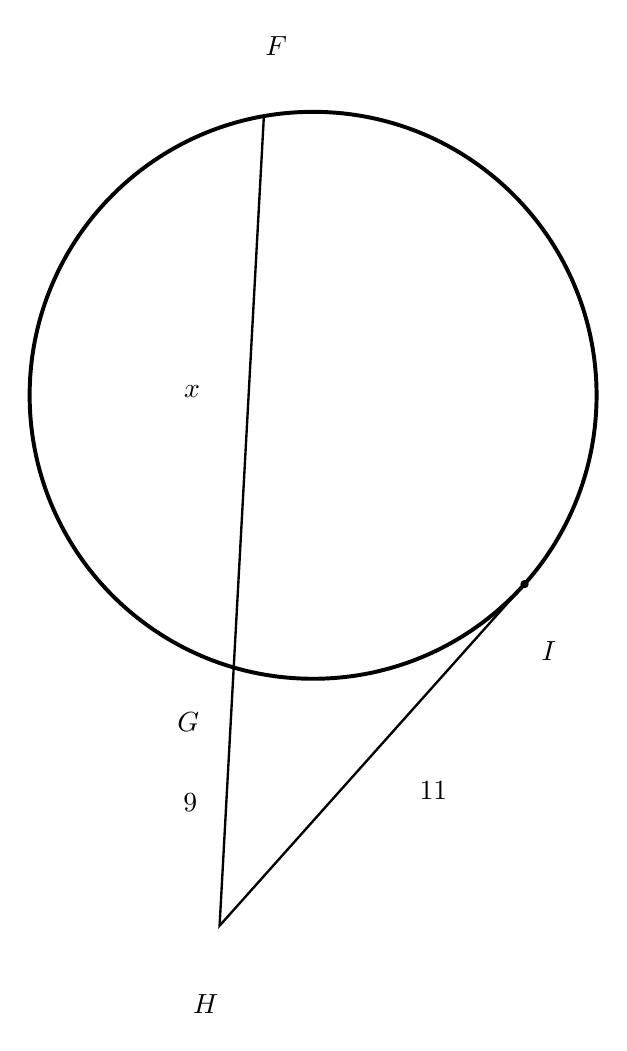
\begin{tikzpicture}[dot/.style={circle, fill=black, inner sep=0pt, outer sep=0pt, minimum size=3pt}, baseline = (current bounding box.west)]

\node[draw,circle,minimum size=2*\radA,inner sep=0pt, line width=0.5mm, outer sep=0] (circ) at (0,0) {};

\path[name path=circum, line width=0.3mm] (circ) circle (\radA);

\coordinate (f) at ($(circ) + (100:\radA)$); 

\coordinate (h) at ($(circ) + (260:1.9*\radA)$); 

\node[dot] (i) at (tangent cs:node=circ, point={(h)}, solution=1) {};  

\draw[name path=line1, line width=0.3mm] (f) -- (h) -- (i) ;

\fill[black, name intersections={of=line1 and circum, name=int}];

\node(g.label) at ($(int-1)+(230:0.25*\radA)$) {$ G$};

\node(f.label) at ($(f)+(80:0.25*\radA)$) {$ F$};

\node(h.label) at ($(h)-(80:0.28*\radA)$) {$ H$};

\node(i.label) at ($(i)+(-70:0.25*\radA)$) {$ I$};

\node(11.label) at ($(h)!0.5!(i) +(-30:0.25*\radA)$) {$ 11$};

\node(9.label) at ($(h)!0.5!(int-1) +(190:0.13*\radA)$) {$ 9$};

\node(x-label) at ($(f)!0.5!(int-1) +(180:0.2*\radA)$) {$ x$}; 

\end{tikzpicture} 
 \\
3. 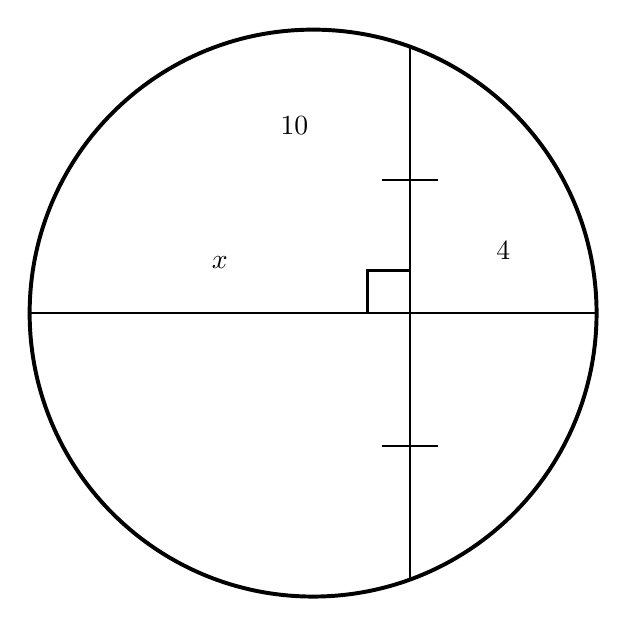
\begin{tikzpicture}[dot/.style={circle, fill=black, inner sep=0pt, outer sep=0pt, minimum size=3pt}, baseline = (current bounding box.west)]

\coordinate (circ) at (0,0); 

\draw[name path=circum, line width=0.5mm] (circ) circle (\radA);

\coordinate (a) at ($(circ) + (180:\radA)$); 

\coordinate (b) at ($(circ) + (0:\radA)$); 

\coordinate (c) at ($(circ) + (70:\radA)$);

\coordinate (d) at ($(circ) + (-70:\radA)$); 

\draw[name path=line1, line width=0.3mm] (a) -- (b);

\draw[name path=line2, line width=0.3mm] (c) -- (d);

\fill[black, name intersections={of=line1 and line2, name=int}];

\begin{scope} [rotate=90]
\draw[line width=0.3mm] (int-1) rectangle ++(0.15*\radA,0.15*\radA) node[transform shape]{};
\end{scope} 

\coordinate (tick1) at ($(c)!0.5!(int-1)$);

\coordinate (tick2) at ($(d)!0.5!(int-1)$); 

\tikzset{onetick/.pic={\draw[line width=0.3mm] ($(0,0)+(0,0.1*\radA)$) -- ($(0,0)-(0,0.1*\radA)$) ; }}

\pic[rotate=90] at (tick1) [pic type = onetick]; 

\pic[rotate=90] at (tick2) [pic type = onetick]; 

\node(10.label) at ($(tick1)+(155:0.45*\radA)$) {$  10$};

\node(4.label) at ($(b)! 0.5!(int-1)+(90:0.22*\radA)$) {$  4$};

\node(x-label) at ($(a)!0.5!(int-1) +(90:0.18*\radA)$) {$  x$}; 

\end{tikzpicture} 
 & 7. \begin{tikzpicture}[dot/.style={circle, fill=black, inner sep=0pt, outer sep=0pt, minimum size=3pt}, baseline = (current bounding box.west)]

\coordinate (circ) at (0,0); 

\draw[name path=circum, line width=0.5mm] (circ) circle (\radA);

\coordinate (l) at ($(circ) + (90:\radA)$); 

\coordinate (k) at ($(circ) + (190:\radA)$);

\coordinate (n) at ($(circ) + (-15:\radA)$); 

\coordinate (j) at ($(l)!2!(k)$); 

\draw[name path=line1, line width=0.3mm] (l) -- (j) -- (n) ;

\fill[black, name intersections={of=line1 and circum, name=int}];

\node(m.label) at ($(int-3)+(-100:0.33*\radA)$) {$ M$};

\node(l.label) at ($(l)+(90:0.25*\radA)$) {$ L$};

\node(j.label) at ($(j)+(220:0.33*\radA)$) {$ J$};

\node(k.label) at ($(k)+(170:0.33*\radA)$) {$ K$};

\node(n.label) at ($(n)+(0:0.25*\radA)$) {$ N$};

\node(x-label) at ($(j)!0.5!(int-3) +(-90:0.2*\radA)$) {$ x$};

\node(10-label1) at ($(j)!0.5!(k) +(180:0.35*\radA)$) {$ 10$};

\node(10-label2) at ($(l)!0.5!(k) +(180:0.2*\radA)$) {$ 10$}; 

\node(8-label) at ($(n)!0.5!(int-3) +(-90:0.25*\radA)$) {$ 8$};

\end{tikzpicture} 
 \\
4. 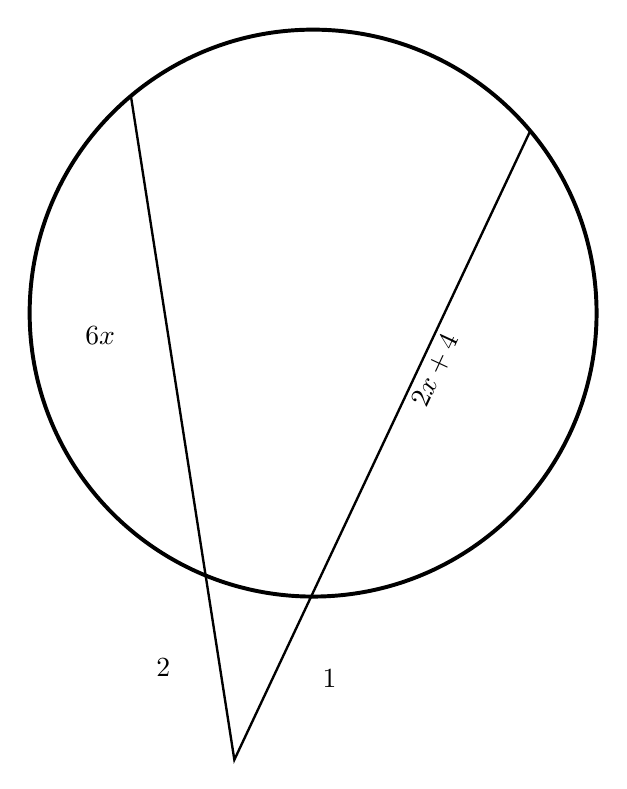
\begin{tikzpicture}[dot/.style={circle, fill=black, inner sep=0pt, outer sep=0pt, minimum size=3pt}, baseline = (current bounding box.west)]

\coordinate (circ) at (0,0); 

\draw[name path=circum, line width=0.5mm] (circ) circle (\radA);

\coordinate (a) at ($(circ) + (130:\radA)$); 

\coordinate (b) at ($(circ) + (260:1.6*\radA)$); 

\coordinate (c) at ($(circ) + (40:\radA)$); 

\draw[name path=line1, line width=0.3mm] (a) -- (b) -- (c) ;

\fill[black, name intersections={of=line1 and circum, name=int}];

\node(2.label) at ($(int-2)! 0.5!(b) + (180:0.2*\radA)$) {$  2$};

\node(1.label) at ($(int-4)! 0.5!(b) + (0:0.2*\radA)$) {$  1$};

\node(6x.label) at ($(int-2)! 0.5!(a) + (180:0.24*\radA)$) {$  6x$};

\node[anchor=north, inner sep=2pt, rotate=65] (2x4.label) at ($(int-4)! 0.5!(c)$) {$  2x+4$};


\end{tikzpicture} 
 & 8. 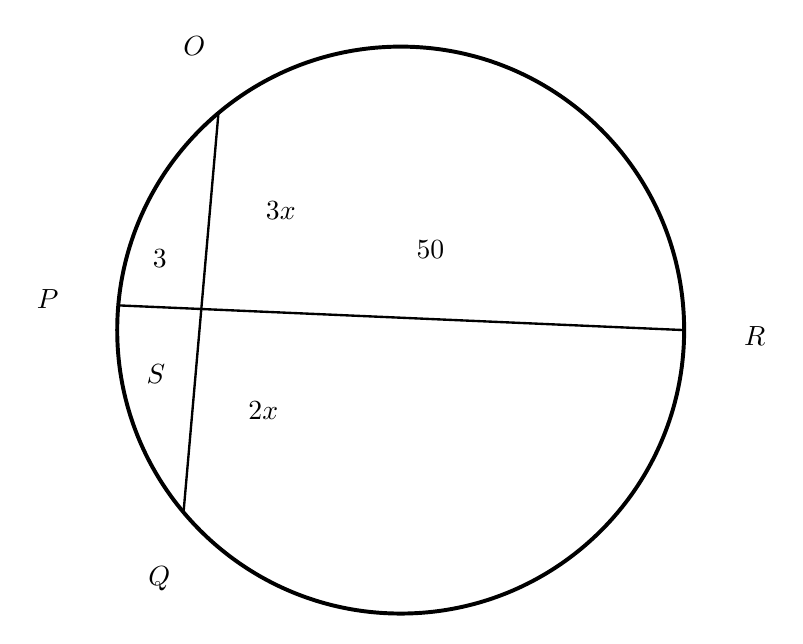
\begin{tikzpicture}[dot/.style={circle, fill=black, inner sep=0pt, outer sep=0pt, minimum size=3pt}, baseline = (current bounding box.west)]

\coordinate (circ) at (0,0); 

\draw[name path=circum, line width=0.5mm] (circ) circle (\radA);

\coordinate (p) at ($(circ) + (175:\radA)$); 

\coordinate (r) at ($(circ) + (0:\radA)$); 

\coordinate (o) at ($(circ) + (130:\radA)$); 

\coordinate (q) at ($(circ) + (220:\radA)$); 

\draw[name path=line1, line width=0.3mm] (p) -- (r) ;

\draw[name path=line2, line width=0.3mm] (o) -- (q)  ;

\fill[black, name intersections={of=line1 and line2, name=int}];

\node(s.label) at ($(int-1)-(55:0.28*\radA)$) {$ S$};

\node(o.label) at ($(o)+(110:0.25*\radA)$) {$ O$};

\node(p.label) at ($(p)+(175:0.25*\radA)$) {$ P$};

\node(q.label) at ($(q)+(250:0.25*\radA)$) {$ Q$};

\node(r.label) at ($(r)+(-5:0.25*\radA)$) {$ R$};

\node(50-label) at ($(r)!0.5!(int-1) +(100:0.25*\radA)$) {$ 50$}; 

\node(3-label) at ($(p)!0.5!(int-1) +(90:0.17*\radA)$) {$ 3$}; 

\node(2x-label) at ($(q)!0.5!(int-1) +(0:0.25*\radA)$) {$ 2x$}; 

\node(3x.label) at ($(o)!0.5!(int-1) +(0:0.25*\radA)$) {$ 3x$};


\end{tikzpicture} 

 \\
\end{tabularx}}
\end{minipage}}
\end{center} 
  

%}} 

%\newpage

%{\fontsize{38}{40}\fontfamily{pnc}\selectfont {

\input{ps-power-theorems-input2}
}}
\newpage

{\fontsize{36}{40}\fontfamily{pnc}\selectfont {
\def\curdir{/storage/emulated/0/Documents/documents/latex/1920/Grade-10/2nd/power-theorems}
\def\radB{1cm}

\textbf{Problem Set}

\vspce

Find the value of $x$. 
\begin{center}
\vspace*{-2ex}
\scalebox{1}{
\noindent\begin{minipage}{\textwidth}
{\begin{tabularx}{\textwidth}{XX}
1. 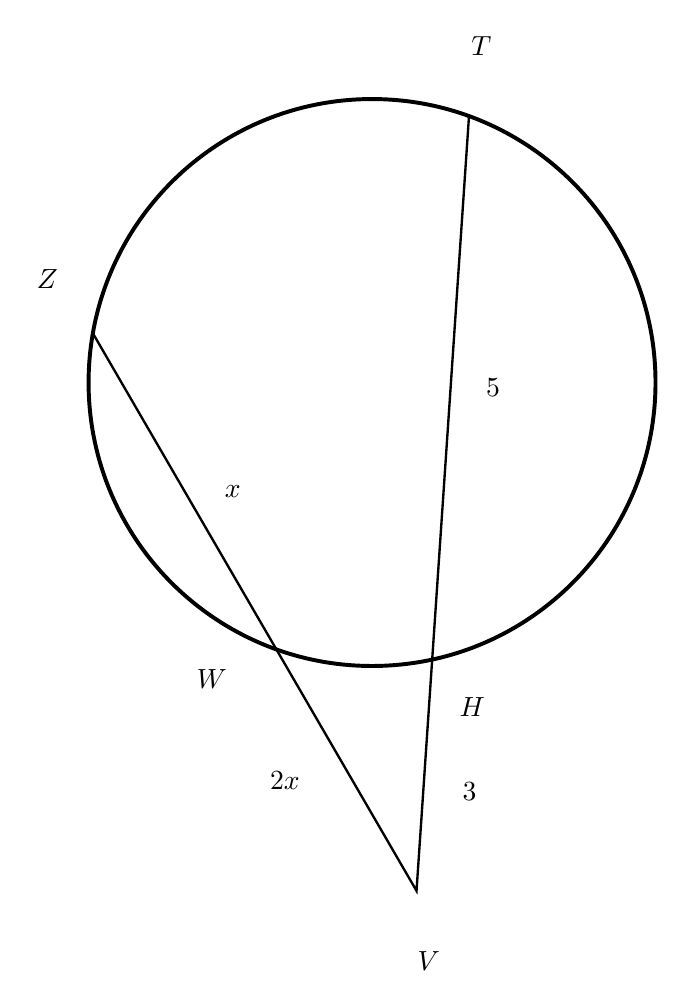
\begin{tikzpicture}[dot/.style={circle, fill=black, inner sep=0pt, outer sep=0pt, minimum size=3pt}, baseline = (current bounding box.west)]

\coordinate (circ) at (0,0); 

\draw[name path=circum, line width=0.5mm] (circ) circle (\radB);

\coordinate (z) at ($(circ) + (170:\radB)$); 

\coordinate (v) at ($(circ) + (275:1.8*\radB)$); 

\coordinate (t) at ($(circ) + (70:\radB)$); 

\draw[line width=0.3mm] (z) -- (v) -- (t) ;

\node(z.label) at ($(z)+(130:0.25*\radB)$) {$ Z$};

\node(t.label) at ($(t)+(80:0.25*\radB)$) {$ T$};

\node(v.label) at ($(v)+(-80:0.25*\radB)$) {$ V$};


\path[name path=linezv, line width=0.3mm] (z) -- (v);

\fill[black, name intersections={of=linezv and circum, name=intzv}];

\node(w.label) at ($(intzv-1)+(205:0.25*\radB)$) {$W$};

\node(x-label) at ($(z)!0.5!(intzv-1)+ (0:0.17*\radB)$) {$x$}; 

\node(2x-label) at ($(v)!0.5!(intzv-1) + (190:0.22*\radB)$) {$ 2x$}; 

\path[name path=linetv, line width=0.3mm] (v) -- (t) ;

\fill[black, name intersections={of=linetv and circum, name=inttv}];

\node(h.label) at ($(inttv-1)+(-50:0.22*\radB)$) {$ H$};

\node(5-label) at ($(t)!0.5!(inttv-1) +(0:0.15*\radB)$) {$ 5$}; 

\node(3-label) at ($(v)!0.5!(inttv-1) +(-20:0.17*\radB)$) {$ 3$}; 



\end{tikzpicture} 
 & 5. 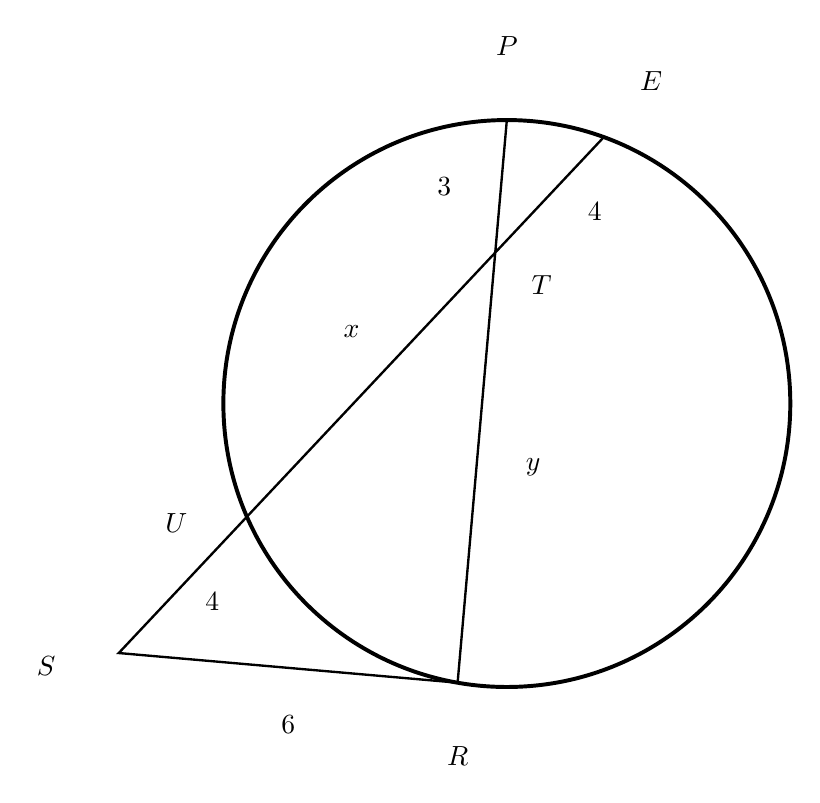
\begin{tikzpicture}[dot/.style={circle, fill=black, inner sep=0pt, outer sep=0pt, minimum size=3pt}, baseline = (current bounding box.west)]

\coordinate (circ) at (0,0); 

\draw[name path=circum, line width=0.5mm] (circ) circle (\radB);

\coordinate (p) at ($(circ) + (90:\radB)$); 

\coordinate (r) at ($(circ) + (260:\radB)$); 

\coordinate (e) at ($(circ) + (70:\radB)$); 

\coordinate (s) at ($(r) + (175:1.2*\radB)$); 

\draw[name path=line1, line width=0.3mm] (p) -- (r) -- (s) -- (e) ;


\path[name path=line2, line width=0.3mm] (s) -- (e) ;

\fill[black, name intersections={of=line1 and line2, name=intt}];

\node(t.label) at ($(intt-1)+(-35:0.2*\radB)$) {$ T$};

\fill[black, name intersections={of=line2 and circum, name=intu}];

\node(u.label) at ($(intu-1)+(185:0.25*\radB)$) {$ U$};

\node(p-label) at ($(p)+(90:0.26*\radB)$) {$ P$}; 

\node(e-label) at ($(e)+(50:0.26*\radB)$) {$ E$}; 

\node(r-label) at ($(r)+(-90:0.26*\radB)$) {$ R$}; 

\node(s-label) at ($(s)+(190:0.26*\radB)$) {$ S$}; 

\node(3-label) at ($(p)!0.5!(intt-1) +(180:0.2*\radB)$) {$ 3$}; 

\node(4-label) at ($(e)!0.5!(intt-1) +(-20:0.17*\radB)$) {$ 4$}; 

\node(x-label) at ($(intu-1)!0.5!(intt-1) +(110:0.2*\radB)$) {$ x$}; 

\node(y-label) at ($(r)!0.5!(intt-1) +(0:0.2*\radB)$) {$ y$}; 

\node(6-label) at ($(s)!0.5!(r) +(-90:0.2*\radB)$) {$ 6$}; 

\node(4-label) at ($(s)!0.5!(intu-1)+(-30:0.12*\radB)$) {$ 4$}; 

\end{tikzpicture} 
 \\
2. \begin{tikzpicture}[dot/.style={circle, fill=black, inner sep=0pt, outer sep=0pt, minimum size=3pt}, baseline = (current bounding box.west)]

\coordinate (circ) at (0,0); 

\draw[name path=circum, line width=0.5mm] (circ) circle (\radB);

\coordinate (r) at ($(circ) + (120:\radB)$); 

\coordinate (n) at ($(circ) + (0:1.6*\radB)$); 

\coordinate (e) at ($(circ) + (210:\radB)$); 

\draw[name path=line1, line width=0.3mm] (r) -- (n) -- (e) ;

\fill[black, name intersections={of=line1 and circum, name=int}];

\node(i.label) at ($(int-1)+(60:0.25*\radB)$) {$ I$};

\node(r-label) at ($(r)+(160:0.25*\radB)$) {$ R$}; 

\node(n-label) at ($(n)+(0:0.25*\radB)$) {$ N$};

\node(e-label) at ($(e)+(-150:0.25*\radB)$) {$ E$};  

\node(g.label) at ($(int-4)+(-40:0.2*\radB)$) {$ G$};

\node(x-label) at ($(r)!0.5!(int-1) +(90:0.17*\radB)$) {$ x$}; 

\node(3-label) at ($(n)!0.5!(int-1) +(70:0.25*\radB)$) {$ 3$}; 

\node(5-label) at ($(e)!0.5!(int-4) +(-90:0.25*\radB)$) {$ 5$}; 

\node(4-label) at ($(n)!0.5!(int-4) +(-70:0.25*\radB)$) {$ 4$}; 

\end{tikzpicture} 

 & 6. 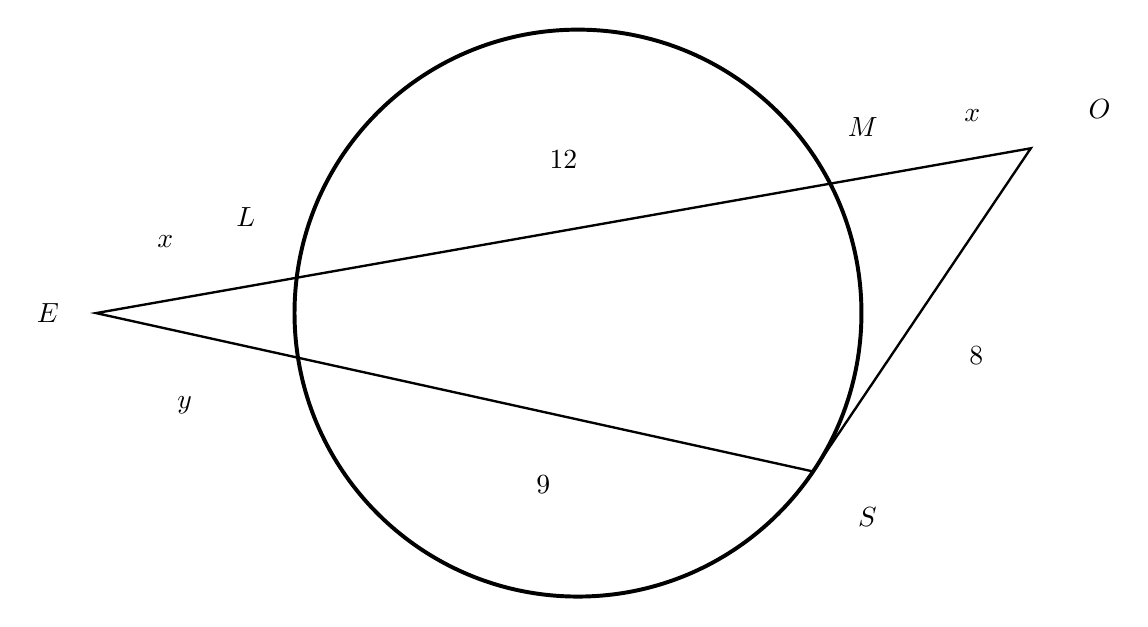
\begin{tikzpicture}[dot/.style={circle, fill=black, inner sep=0pt, outer sep=0pt, minimum size=3pt}, baseline = (current bounding box.west)]

\node[draw,circle,minimum size=2*\radB,inner sep=0pt, line width=0.5mm, outer sep=0] (circ) at (0,0) {};

\path[name path=circum, line width=0.5mm] (circ) circle (\radB);

\coordinate (e) at ($(circ) + (180:1.7*\radB)$); 

\coordinate (o) at ($(circ) + (20:1.7*\radB)$); 

\coordinate (s) at (tangent cs:node=circ, point={(o)}, solution=2);  

\draw[name path=line1, line width=0.3mm] (e) -- (o) -- (s) -- cycle ;

\path[name path=line2, line width=0.3mm] (e) -- (o) ;

\fill[black, name intersections={of=line2 and circum, name=int}];

\node(l.label) at ($(int-2)+(130:0.28*\radB)$) {$ L$};

\node(e.label) at ($(e)+(180:0.17*\radB)$) {$ E$};

\node(o.label) at ($(o)+(30:0.28*\radB)$) {$ O$};

\node(s.label) at ($(s)+(-40:0.25*\radB)$) {$ S$};

\node(m.label) at ($(int-1)+(60:0.23*\radB)$) {$ M$};

\node(12-label) at ($(int-1)!0.5!(int-2) +(90:0.25*\radB)$) {$ 12$};

\node(x-label) at ($(e)!0.5!(int-2) +(120:0.22*\radB)$) {$ x$}; 

\node(x2-label) at ($(o)!0.5!(int-1) +(50:0.23*\radB)$) {$ x$}; 

\path[name path=line3, line width=0.3mm] (e) -- (s) ;

\fill[black, name intersections={of=line3 and circum, name=int}];

\node(y-label) at ($(e)!0.5!(int-1) +(-100:0.25*\radB)$) {$ y$};

\node(9-label) at ($(s)!0.5!(int-1) +(-100:0.25*\radB)$) {$ 9$}; 

\node(8-label) at ($(s)!0.5!(o) +(-40:0.25*\radB)$) {$ 8$};

\end{tikzpicture} 
 \\
3. \begin{tikzpicture}[dot/.style={circle, fill=black, inner sep=0pt, outer sep=0pt, minimum size=3pt}, baseline = (current bounding box.west)]

\node[draw,circle,minimum size=2*\radB,inner sep=0pt, line width=0.5mm, outer sep=0] (circ) at (0,0) {};

\coordinate (g) at ($(circ) + (-80:\radB)$); 

\coordinate (n) at ($(circ) + (0:\radB)$); 

\coordinate (o) at ($(n)!-1!(g)$); 

\coordinate (s) at (tangent cs:node=circ, point={(o)}, solution=1);  

\draw[name path=line1, line width=0.3mm] (g) --(n) node[midway] (tick1) {} -- (o) node[midway] (tick2) {} -- (s) ;

\node(g.label) at ($(g)+(-90:0.25*\radB)$) {$ G$};

\node(s.label) at ($(s)+(90:0.25*\radB)$) {$ S$};

\node(o.label) at ($(o)+(30:0.25*\radB)$) {$ O$};

\tikzset{onetick/.pic={\draw[line width=0.3mm] ($(0,0)+(0,0.1*\radB)$) -- ($(0,0)-(0,0.1*\radB)$) ; }}

\pic[rotate=50] at (tick1) [pic type = onetick];  

\pic[rotate=50] at (tick2) [pic type = onetick];  

\node(x.label) at ($(tick1)+(90:0.28*\radB)$) {$ x$};

\node(10-label) at ($(s)!0.5!(o) +(90:0.25*\radB)$) {$ 10$}; 

\end{tikzpicture} 

 & 7. 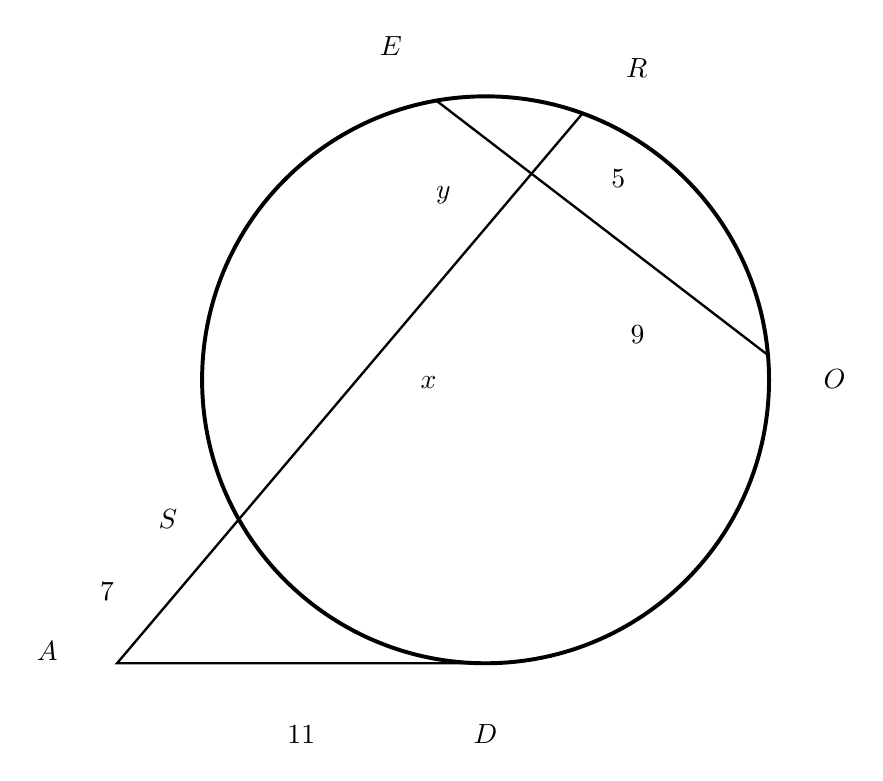
\begin{tikzpicture}[dot/.style={circle, fill=black, inner sep=0pt, outer sep=0pt, minimum size=3pt}, baseline = (current bounding box.west)]

\coordinate (circ) at (0,0); 

\draw[name path=circum, line width=0.5mm] (circ) circle (\radB);

\coordinate (e) at ($(circ) + (100:\radB)$); 

\coordinate (o) at ($(circ) + (5:\radB)$); 

\coordinate (r) at ($(circ) + (70:\radB)$);

\coordinate (d) at ($(circ) + (-90:\radB)$); 

\coordinate (a) at ($(d) + (180:1.3*\radB)$);

\draw[name path=line1, line width=0.3mm] (e) -- (o);

\draw[line width=0.3mm](r) -- (a) -- (d) ;

\path[name path=line2, line width=0.3mm] (r) -- (a);

\fill[black, name intersections={of=line2 and circum, name=ints}];

\node(e.label) at ($(e)+(130:0.25*\radB)$) {$ E$};

\node(s.label) at ($(ints-1)+(180:0.25*\radB)$) {$ S$};

\node(r.label) at ($(r)+(40:0.25*\radB)$) {$ R$};

\node(o.label) at ($(o)+(-20:0.25*\radB)$) {$ O$};

\node(d.label) at ($(d)+(-90:0.25*\radB)$) {$ D$};

\node(11-label) at ($(a)!0.5!(d) +(-90:0.25*\radB)$) {$ 11$}; 

\node(a.label) at ($(a)+(170:0.25*\radB)$) {$ A$};

\fill[black, name intersections={of=line1 and line2, name=int}];

\node(y-label) at ($(e)!0.5!(int-1) +(235:0.25*\radB)$) {$ y$}; 

\node(5-label) at ($(r)!0.5!(int-1) +(-30:0.25*\radB)$) {$ 5$}; 

\node(9-label) at ($(o)!0.5!(int-1) +(260:0.25*\radB)$) {$ 9$}; 

\node(x-label) at ($(ints-1)!0.5!(int-1) +(-40:0.2*\radB)$) {$ x$}; 

\node(7-label) at ($(a)!0.5!(ints-1) +(180:0.25*\radB)$) {$ 7$}; 

\end{tikzpicture} 

 \\
4.  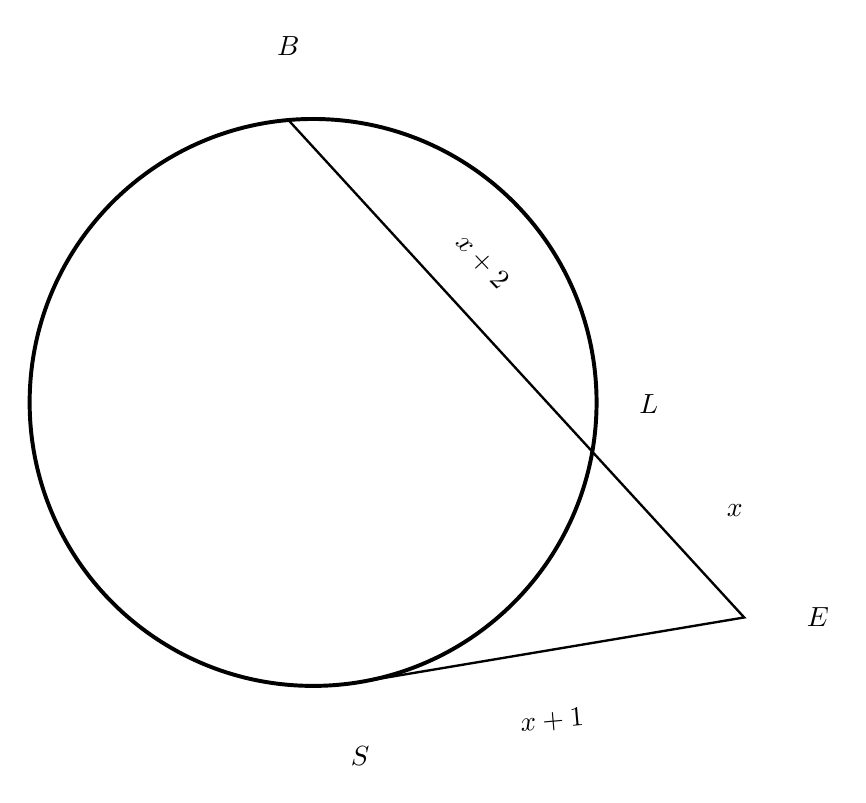
\begin{tikzpicture}[dot/.style={circle, fill=black, inner sep=0pt, outer sep=0pt, minimum size=3pt}, baseline = (current bounding box.west)]

\node[draw,circle,minimum size=2*\radB,inner sep=0pt, line width=0.5mm, outer sep=0] (circ) at (0,0) {};

\coordinate (b) at ($(circ) + (95:\radB)$); 

\coordinate (l) at ($(circ) + (-10:\radB)$); 

\coordinate (e) at ($(l)! -0.5! (b)$); 

\coordinate (s) at (tangent cs:node=circ, point={(e)}, solution=2);  

\draw[name path=line1, line width=0.3mm] (b) -- (l) node[midway] (tick1) {} -- (e) node[midway] (tick2) {}  -- (s) node[midway] (tick3) {} ;

\node(b.label) at ($(b)+(90:0.26*\radB)$) {$ B$};

\node(l.label) at ($(l)+(40:0.26*\radB)$) {$ L$};

\node(e.label) at ($(e)+(0:0.26*\radB)$) {$ E$};

\node(s.label) at ($(s)+(-90:0.26*\radB)$) {$ S$};

\node[rotate=-47](x2.label) at ($(tick1)+(30:0.17*\radB)$) {$ x+2$};

\node(x-label) at ($(tick2) +(20:0.25*\radB)$) {$ x$};

\node[rotate=5](x1-label) at ($(tick3) +(-90:0.25*\radB)$) {$ x+1$}; 

\end{tikzpicture} 

 & \\
\end{tabularx}}
\end{minipage}}
\end{center} 
  

}}
\newpage

{\fontsize{36}{40}\fontfamily{pnc}\selectfont {
\input{ps-power-theorems-sol}

}}

\end{document}